% fig_roadmap: a flowchart of the proof of the main theorem.
% Build: latexmk -pdf fig_roadmap.tex (build.sh copies the PDF to ../).
\documentclass[10pt,border=2pt]{standalone}
\usepackage{amsmath,amssymb}
\usepackage{tikz}
\usetikzlibrary{calc,arrows.meta}

% the palette of the other figures (Okabe-Ito highlights)
\definecolor{ink}{HTML}{1A1A1A}
\definecolor{muted}{HTML}{555555}
\definecolor{ringfill}{HTML}{DCE3EB}
\definecolor{ringedge}{HTML}{8E9DAD}
\definecolor{hlorange}{HTML}{D55E00}
\definecolor{orangetint}{HTML}{F6D5BF}

\newcommand{\sect}[1]{\enspace{\footnotesize\color{muted}(\S#1)}}

\begin{document}
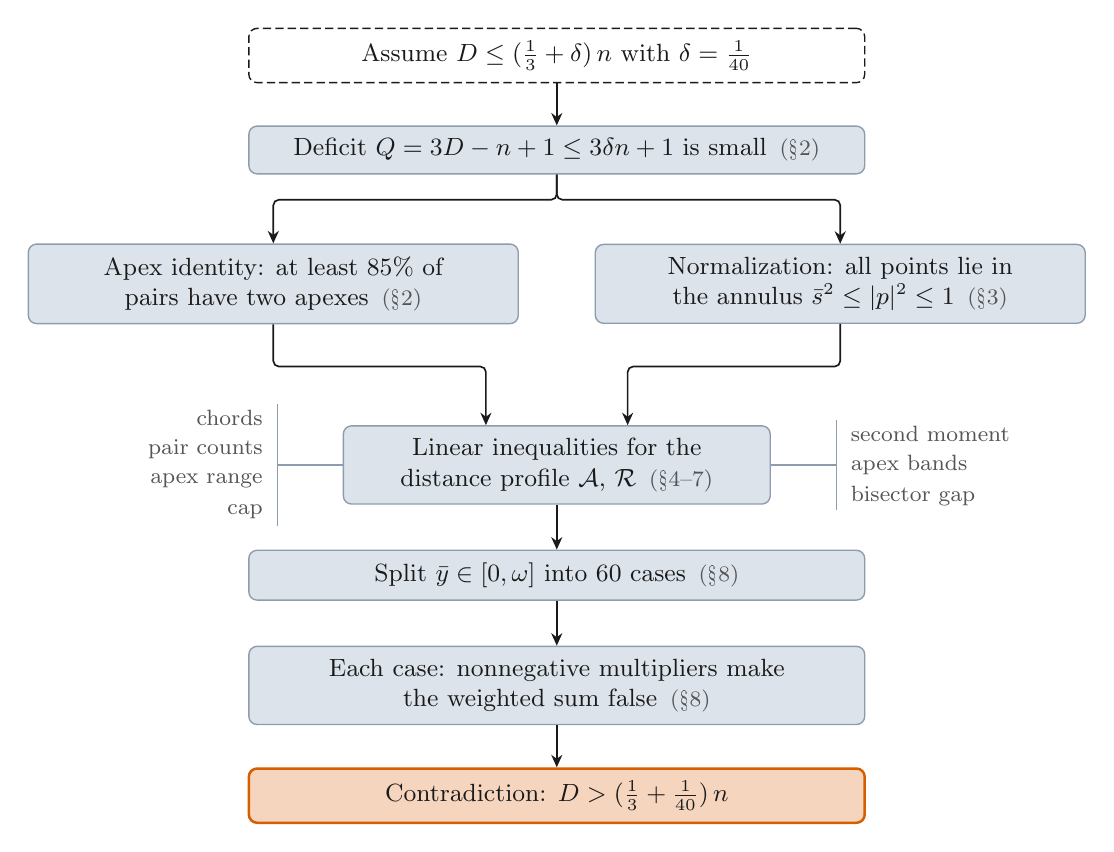
\begin{tikzpicture}[
    x=1mm, y=1mm,
    font=\small,
    box/.style={draw=ringedge, fill=ringfill, rounded corners=3pt,
      line width=0.5pt, align=flush center, inner xsep=6pt, inner ysep=4.5pt,
      text=ink},
    hyp/.style={box, draw=ink, fill=white, dash pattern=on 3pt off 1.5pt},
    goal/.style={box, draw=hlorange, fill=orangetint, line width=0.9pt},
    fam/.style={font=\footnotesize, text=muted, inner sep=0.8pt},
    arr/.style={-{Stealth[length=4.5pt,width=4pt]}, line width=0.6pt,
      draw=ink, rounded corners=2pt},
    link/.style={line width=0.45pt, draw=ringedge},
  ]
  % ---- main boxes
  \node[hyp, text width=74mm] (assume) at (0, 0)
    {Assume $D \le (\tfrac13+\delta)\,n$ with $\delta = \tfrac1{40}$};
  \node[box, text width=74mm] (deficit) at (0, -12)
    {Deficit $Q = 3D - n + 1 \le 3\delta n + 1$ is small\sect{2}};
  \node[box, text width=58mm] (apex) at (-36, -29)
    {Apex identity: at least $85\%$ of\\ pairs have two apexes\sect{2}};
  \node[box, text width=58mm] (annulus) at (36, -29)
    {Normalization: all points lie in\\ the annulus $\bar s^2 \le |p|^2 \le 1$\sect{3}};
  \node[box, text width=50mm] (ineq) at (0, -52)
    {Linear inequalities for the\\ distance profile $\mathcal A$, $\mathcal R$\sect{4--7}};
  \node[box, text width=74mm] (split) at (0, -66)
    {Split $\bar y \in [0, \omega]$ into $60$ cases\sect{8}};
  \node[box, text width=74mm] (farkas) at (0, -80)
    {Each case: nonnegative multipliers make\\ the weighted sum false\sect{8}};
  \node[goal, text width=74mm] (contra) at (0, -94)
    {Contradiction: $D > (\tfrac13 + \tfrac1{40})\,n$};

  % ---- the inequality families, as side labels of (ineq)
  \foreach \lab [count=\i] in {chords, pair counts, apex range, cap}
    \node[fam, anchor=east] at (-37, -46.0 - 4*\i + 4) {\lab};
  \foreach \lab [count=\i] in {second moment, apex bands, bisector gap}
    \node[fam, anchor=west] at (37, -48.0 - 4*\i + 4) {\lab};
  \draw[link] (-35.5, -44.3) -- (-35.5, -59.7);
  \draw[link] (-35.5, -52) -- (ineq.west);
  \draw[link] (35.5, -46.3) -- (35.5, -57.7);
  \draw[link] (35.5, -52) -- (ineq.east);

  % ---- arrows
  \draw[arr] (assume) -- (deficit);
  \draw[arr] (deficit.south) -- ++(0, -3.2) -| (apex.north);
  \draw[arr] (deficit.south) -- ++(0, -3.2) -| (annulus.north);
  \draw[arr] (apex.south) |- (-9, -39.5) -- (-9, -52 |- ineq.north);
  \draw[arr] (annulus.south) |- (9, -39.5) -- (9, -52 |- ineq.north);
  \draw[arr] (ineq) -- (split);
  \draw[arr] (split) -- (farkas);
  \draw[arr] (farkas) -- (contra);
\end{tikzpicture}
\end{document}
